\section{Scaling Up}

For the moment, we always made one big assumption: {\bf All data fits on a single server}. Even more, all data fits in the memory. It's a realistic assumption for \emph{prototyping}. But it becomes totally obsolete when moving to production. In this chapter, we will introduce the Big Data Problem as well as Spark.

\subsection{Big Data Problem}
Nowadays, Internet is the biggest source of data. And it is growing faster and faster. Even if computers are really powerful, Data Scientist encounters one problem: The Big Data Problem. Indeed, {\bf Data is growing faster than computation speeds}. 

We can see, for example, that CPU speed is stalling and that there is a bottleneck in storage. Therefore a single machine can no longer process or even store all the data. The only solution is to {\bf ditribute} data over large clusters.

\subsubsection{How much data do you need?}
The answer depends on the question. But for many applications the answer is: {\bf as much as we can get}. Big Data about people (text, web, social media, etc.) follow the power law statistics. Indeed, most of the features occur only once or twice. Therefore the distribution is a long tail distribution. And the long tail is really important. For example, Google knows that you're looking for something even if you checked on the web once or twice.

The number of features grows in proportion to the amount of data, {\it i.e.} doubling the dataset size roughly doubles the number of users we observe. Therefore, even one or two observations of a user improves predictions for them, so:
\begin{center}
 {\bf More data and bigger models $=>$ More revenue!}
\end{center}

\subsubsection{Hardware for Big Data}
At the beginning, Google (and other Internet companies) used many low-end servers instead of expensive high-end servers. It is easier to add capacity and it is cheaper per CPU/disk. But there are problems:
\begin{itemize}
 \item {\bf Failures} (e.g. Google numbers)
 \begin{itemize}
  \item 1-5\% hard drives/year
  \item 0.2\% DIMMs/year (RAM)
 \end{itemize}
 \item {\bf Commodity Network} (1-20 Gb/s) speed vs RAM
 \begin{itemize}
  \item Much more latency (100x -- 100000x)
  \item Lower throughput (100x-1000x)
 \end{itemize}
 \item {\bf Uneven Performance}
 \begin{itemize}
  \item Inconsistent hardware skew
  \item Variable network latency
  \item External loads
 \end{itemize}
\end{itemize}

\begin{center}
{\bf These numbers are constantly changing thanks to new technology!}
\end{center}

\subsubsection{How do we split work across machines? (Map-Reduce)}

\begin{center}
\emph{How do you count the number of occurences of each word in a document?}
\end{center}

We can use a {\bf hash table}. It's an easy tool to use for these kind of task. But what happens if the document is really big? (For example, the web) We can simple {\bf chunk} the document into multiple documents and create a hash table on each machines. At the end, we aggregate all the hash tables. {\bf But} the machine that aggregates is the {\bf bottleneck} in term of performance. And if this machine crashes, it's a disaster!

\begin{figure}[H]%---------------FIG--------------
 \centering
 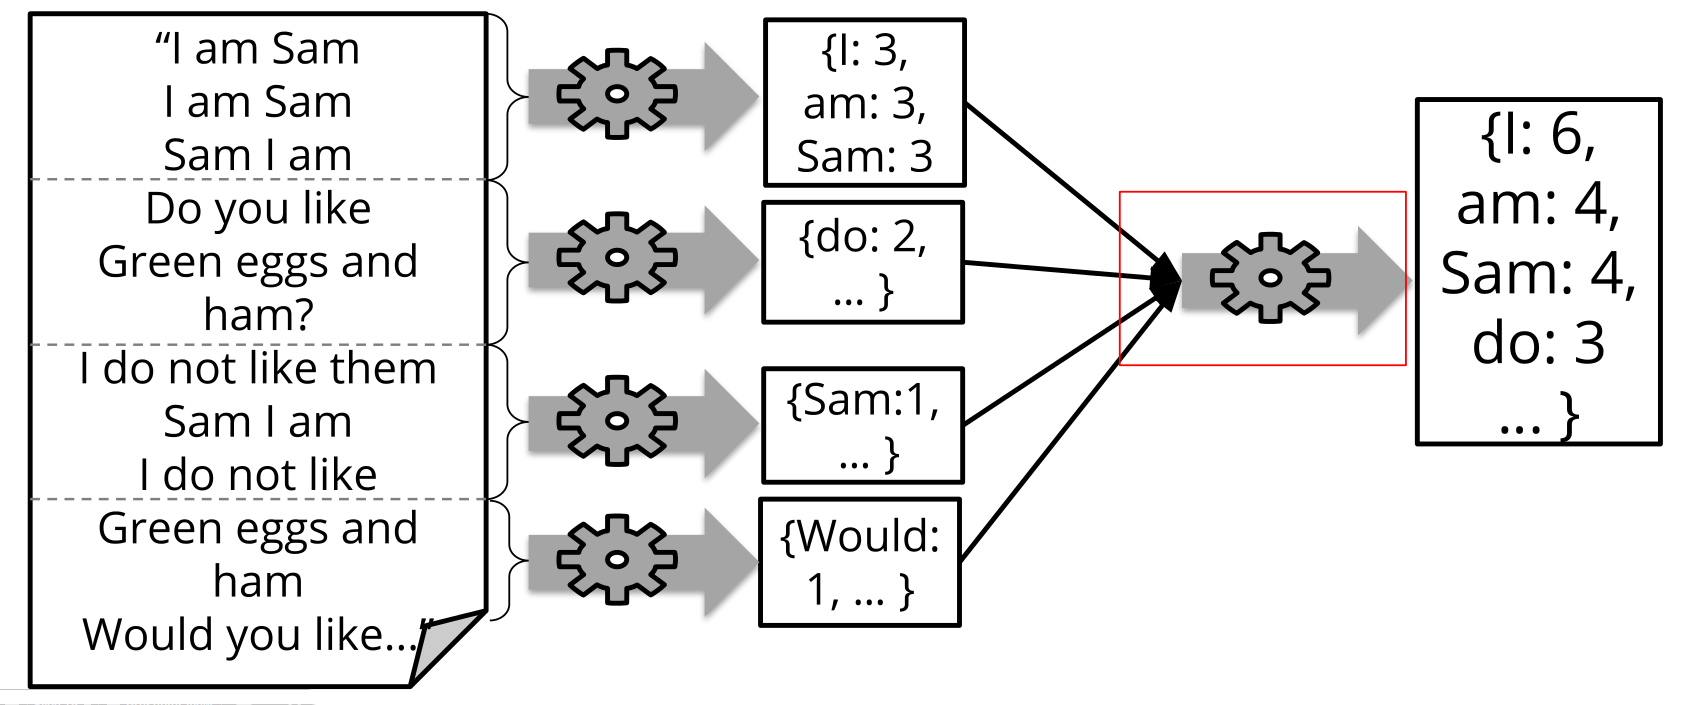
\includegraphics[width=13cm]{./img/10/hash-table}
 \caption{\label{pic:hash-table} Usage of hash tables on multiple machines. We see that the bottleneck machine is the machine that aggregates the hash tables into one.}
\end{figure}

Therefore, we can use a more clever algorithm: {\bf Divide-and-Conquer}. Each node is responsible os summing up a subset of the whole hash table. 

\begin{figure}[H]%---------------FIG--------------
 \centering
 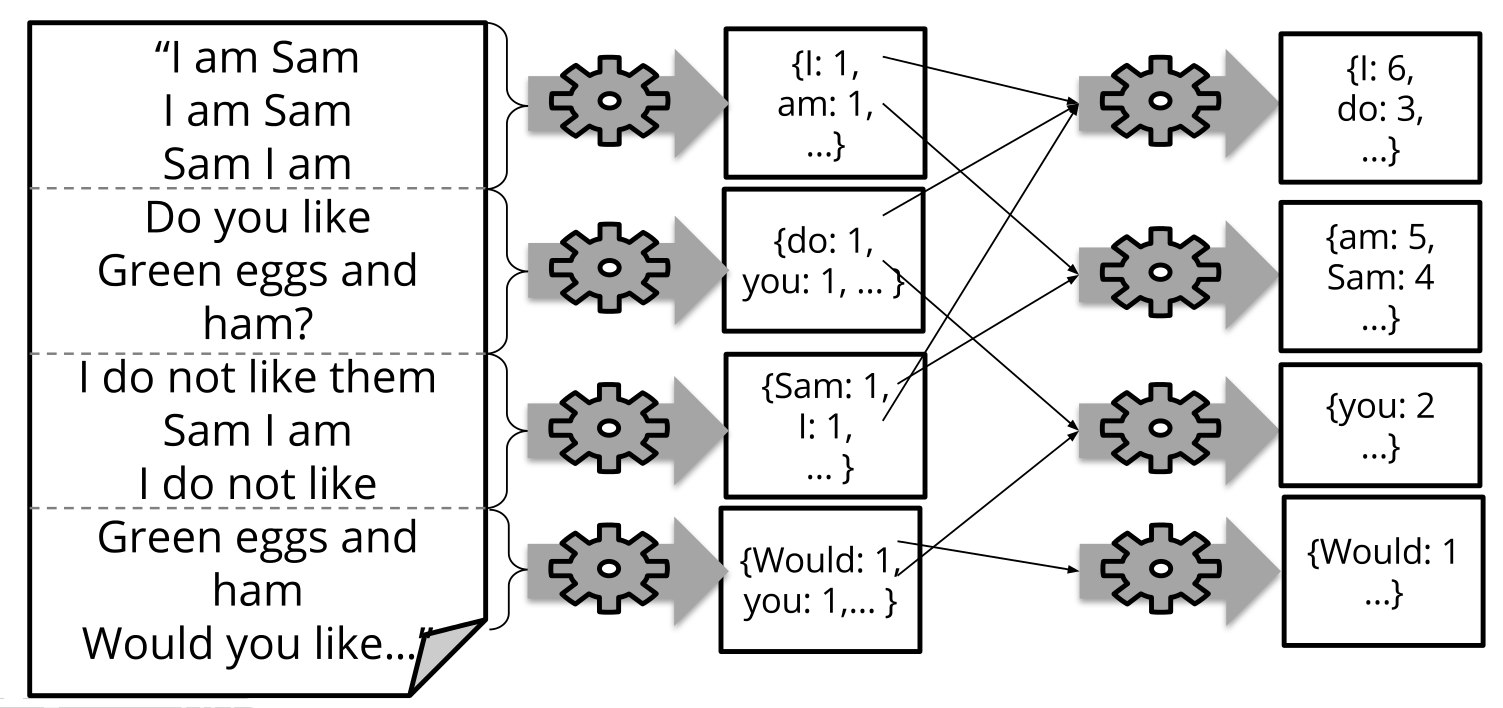
\includegraphics[width=13cm]{./img/10/divide-and-conquer}
 \caption{\label{pic:divide-and-conquer} Usage of hash tables on multiple machines with Divide-and-Conquer technique. We don't have any bottleneck this time.}
\end{figure}

This technique is called {\bf Map Reduce}. The first part is called map because we create a map for each part of the big document. Then we reduce it into a simpler hash table. This works well when using a lot of different nodes. In addition, each task is {\bf idem-potent}. It means that the order of the word count doesn't matter. Thus, it is really easy to user without waiting the other nodes to finish.

\begin{figure}[H]%---------------FIG--------------
 \centering
 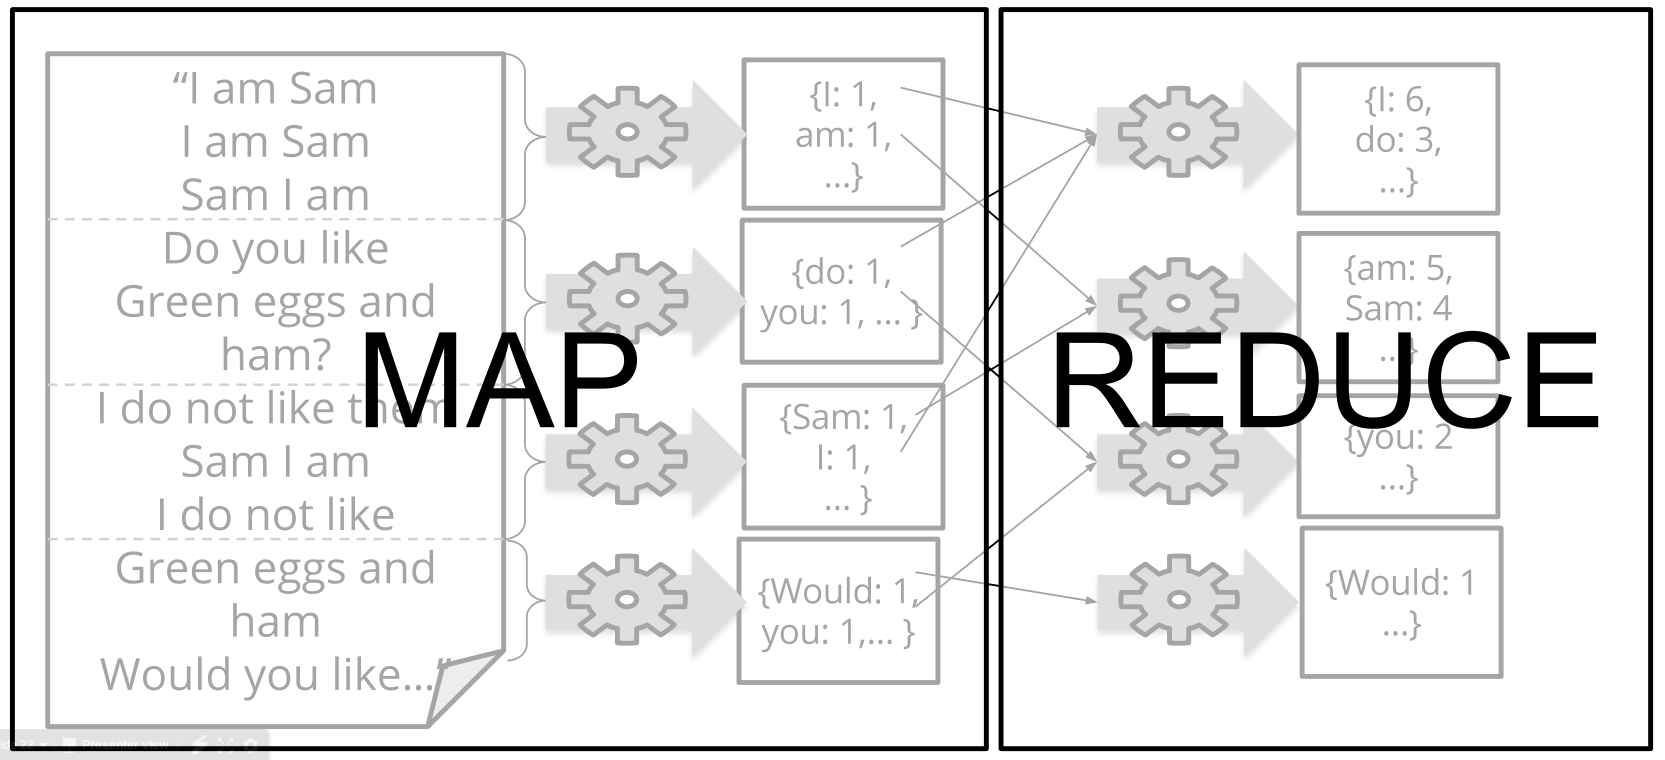
\includegraphics[width=13cm]{./img/10/map-reduce}
 \caption{\label{pic:map-reduce} Map Reduce illustrated on the Divide-and-Conquer algorithm in Figure \ref{pic:divide-and-conquer}}
\end{figure}

\paragraph{What's hard about cluster computing?}

How to divide work across machines?
\begin{itemize}
 \item We Must consider network, data locality. (It's always better on its own machine.)
 \item Moving data may be {\bf very} expensive!
\end{itemize}

How to deal with failures?
\begin{itemize}
 \item 1 server fails every 3 years. Therefore, 10K nodes will give 10 faults/day.
 \item Even worse: stragglers. The node has not failed but is slow.
\end{itemize}

How to deal with failures? {\bf Just launch another task!}

\begin{figure}[H]%---------------FIG--------------
 \centering
 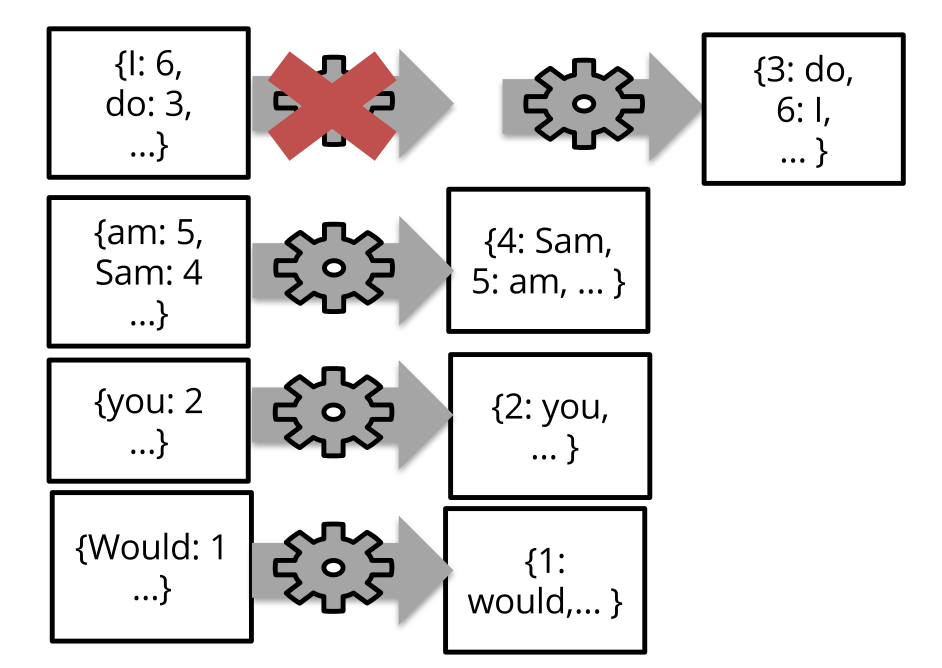
\includegraphics[width=13cm]{./img/10/failure}
 \caption{\label{pic:failure} To deal with failure, we can just launch another task.}
\end{figure}

Large Parallel Databases did not support fault tolerance until recently. Therefore, if the query fails you have to redo it since the beginning. For example, if the query takes longer than 3 hours you will experience one failure on a server during the query. Thus, the query is useless.

How to deal with slow tasks? {\bf Just launch another task!}

\begin{figure}[H]%---------------FIG--------------
 \centering
 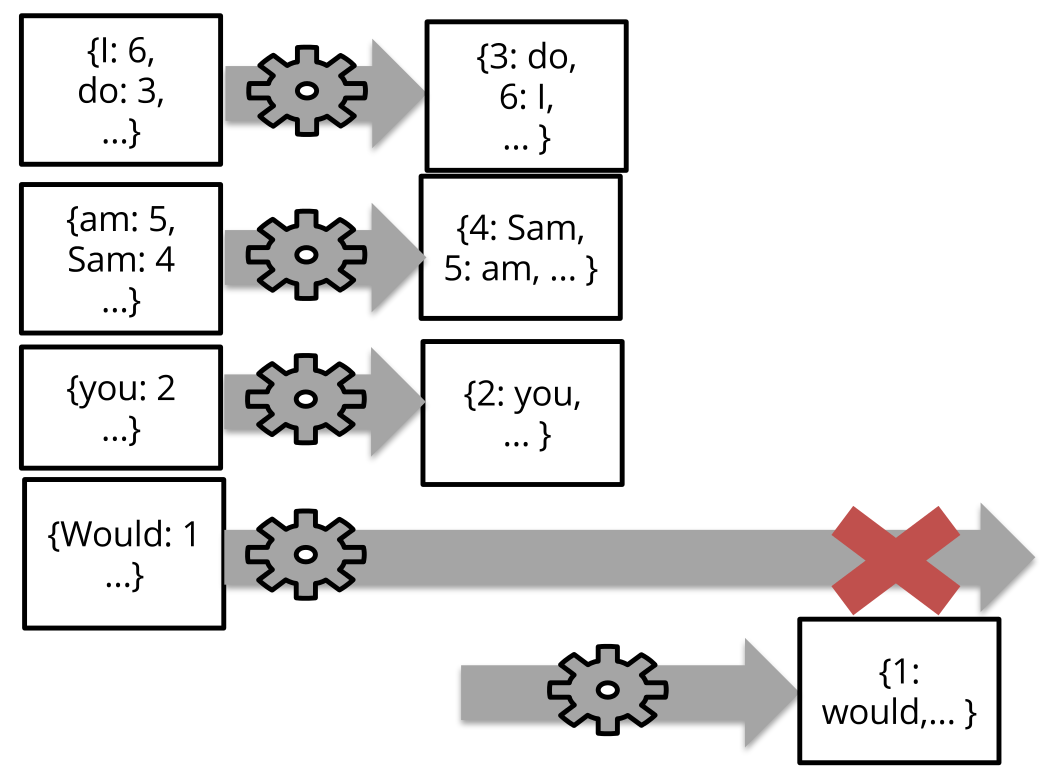
\includegraphics[width=13cm]{./img/10/slow}
 \caption{\label{pic:failure} To deal with slow tasks, we can just launch another task.}
\end{figure}

Map-Reduce is not used by Google anymore, even if they invented it. More advance techniques exist nowadays. Why? Because Memory is really cheap! (RAM: 1 cent/Mb)

\subsection{Spark Computing Framework}

Spark provides a programming abstraction and parallel runtime to hide all of these complexity. Table \ref{tab:spark-hadoop} shows the main differences between Spark and Hadoop Map-Reduce. The big advantage with Spark is that it deals itself with all the complex clustering between the nodes.

\begin{table}[H]
 \begin{center}
  \begin{tabular}{l|l|l}
    & Hadoop Map Reduce & Apache Spark \\ \hline \hline
    Storage & Disk only & In-memory or on disk \\ \hline
    Operations & Map and Reduce & Map, Reduce, Join, Sample, etc. \\ \hline
    Ease of use & Java program & Scala and Python shells \\ \hline
  \end{tabular}
 \end{center}
 \caption{\label{tab:spark-hadoop} Main differences between Spark and Hadoop}
\end{table}

One of the big advantage of Spark is that it uses in-memory storage. This can speed-up the computation time by a factor of 100 on the Logistic Regression for example. The good thing with Spark is that if the RAM is full, then it will use the memory on disk. We can see some interesting fact about having data {\bf in-memory}:
\begin{itemize}
 \item Optimized for batch, data-parallel ML algorithms
 \item An efficient, general-purpose language for cluster processing of big data
 \item In-memory query processing (Spark SQL)
\end{itemize}

Spark is not only good because it's faster than Hadoop. For example, we can see that some practical Challenges with Hadoop are:
\begin{itemize}
 \item Very {\bf low-level} programming model
 \item Very {\bf little re-use} of Map-Reduce code between applications
 \item {\bf Laborious} programming: design code, build jar, deploy on cluster
 \item {\bf Relies heavily on Java reflection} to communicate with to-be-defined application code.
\end{itemize}

And some practical Advantages of Spark are:
\begin{itemize}
 \item {\bf High-level programming model}: can be used like SQL (Dataframe) or like a tuple store.
 \item {\bf Interactivity}
 \item {\bf Integrated UDFs} (User-Defined Functions)
 \item High-level model ({\bf Scala Actors}) for distributed programming
 \item {\bf Scala generics} instead of reflection: Spark code is generic over [Key, Value] types.
\end{itemize}

One last advantage of Spark is the way it deal with {\bf Fault tolerance}. Hadoop uses data replication on \href{https://en.wikipedia.org/wiki/Apache\_Hadoop#HDFS}{HDFS}. Therefore, once it's computed, you should not loose it. On the other hand, Spark remember {\bf how} to recompute everything. For example, it will remember which nodes failed and which road he used to compute everything.

\subsubsection{Read more}

If you want to read more on Haddop, you can go on \href{http://hadoop.apache.org/}{Apache Hadoop website}. For Spark, you can go on \href{http://spark.apache.org/}{Aparche Spark website}. A good article comparing Spark and Hadoop can be found on \href{https://www.xplenty.com/blog/2014/11/apache-spark-vs-hadoop-mapreduce/}{Xplenty}. You can always find more information about Spark and Hadoop on Internet. But the thing you should know is that even if Spark is much faster and much easier to use, Hadoop is not ready yet for the \emph{elephant's graveyard}.